\documentclass[tikz]{standalone}
\usetikzlibrary{shapes.geometric}    % trapezium
\usetikzlibrary{arrows}              % arrow tips
\usepackage{amsmath}
\usepackage{bm}                      % boldsymbol
\usepackage{makecell}                % makecell
\begin{document}
    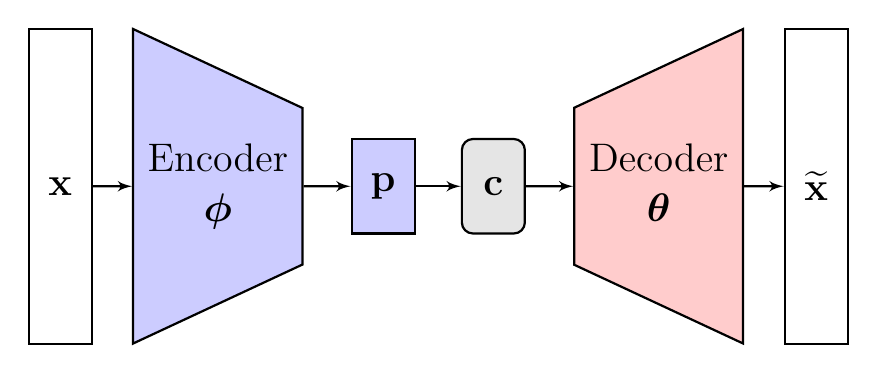
\begin{tikzpicture}[baseline=0, >=latex',thick]
      \node (rect) at (0,0)
      [draw, thick, minimum width=0.8cm, minimum height=4cm, name=x]
      {\Large{$\textbf{x}$}};

      \node [trapezium, trapezium angle=65, minimum width=4cm,
      inner xsep=0.3cm,
      draw, thick, rotate=-90, fill=blue!20, name=enc] at (2,0)
      {\rotatebox{90}{\Large{\makecell[c]{Encoder\\$\boldsymbol{\phi}$}}}};

      \draw [->] (x) -- (enc);

      \node (rect) at (4.1,0)
      [draw, thick, minimum width=0.8cm, minimum height=1.2cm, name=sigma, fill=blue!20,
      label={[yshift=-2.5cm]\large{\makecell[c]{}}}, name=p]
      {\Large{$\textbf{p}$}};

      \draw [->] (enc) -- (p);

      \node [rectangle, rounded corners] at (5.5,0)
      [draw, thick, minimum width=0.8cm, minimum height=1.2cm, name=sigma, fill=gray!20,
      label={[yshift=-2.5cm]\large{\makecell[c]{}}}, name=c]
      {\Large{$\textbf{c}$}};

      \draw [->] (p) -- (c);

      \node [trapezium, trapezium angle=65, minimum width=4cm,
      inner xsep=0.3cm, name=dec,
      draw, thick, rotate=90, fill=red!20] at (7.6,0)
      {\rotatebox{-90}{\Large{\makecell[c]{Decoder\\$\boldsymbol{\theta}$}}}};

      \draw [->] (c) -- (dec);

      \node (rect) at (9.6,0)
      [draw, thick, minimum width=0.8cm, minimum height=4cm, name=xt]
      {\Large{$\widetilde{\textbf{x}}$}};

      \draw [->] (dec) -- (xt);
    \end{tikzpicture}
\end{document}
